\R has many built-in functions, and many more in external packages. We will introduce them as we go, but let's get started with some basic ones.
The documentation on each function can be obtained by using \code{?func} or \code{help(func)} where \texttt{func} is some function. For example, to get the documentation about using the \code{help()} function, try the following:
\begin{knitrout}
\definecolor{shadecolor}{rgb}{0.969, 0.969, 0.969}\color{fgcolor}\begin{kframe}
\begin{alltt}
\hlkwd{help}\hlstd{(help)}
\hlopt{?}\hlstd{help}
\end{alltt}
\end{kframe}
\end{knitrout}

When we start an \R session, it's important to determine the `working directory'. This is the folder on our computer which \R will use to search for data or code files and save results. To find out which folder is currently used, we use the \code{getwd()} function
\begin{knitrout}
\definecolor{shadecolor}{rgb}{0.969, 0.969, 0.969}\color{fgcolor}\begin{kframe}
\begin{alltt}
\hlkwd{getwd}\hlstd{()}
\end{alltt}
\begin{verbatim}
[1] "/Users/runner/work/sids/sids/book/Rnw"
\end{verbatim}
\end{kframe}
\end{knitrout}

If we want (and we often will), we may change the working directory by using \code{setwd()}.  
\begin{knitrout}
\definecolor{shadecolor}{rgb}{0.969, 0.969, 0.969}\color{fgcolor}\begin{kframe}
\begin{alltt}
\hlkwd{setwd}\hlstd{(}\hlstr{"~/Desktop"}\hlstd{)}
\end{alltt}
\end{kframe}
\end{knitrout}
The \verb|~/| notation is a shortcut to your home directory. Using this shortcut is convenient because if you are using different computers or you share code with others, the home directory may be different on each computer.

Data is stored in variables. We can get the data from a file (Excel, comma-separated values, etc.), the Internet, or we can generate it ourselves. Let's start by generating some data.
The simplest function to create data is called \code{c()}, which stands for `combine'.
\begin{knitrout}
\definecolor{shadecolor}{rgb}{0.969, 0.969, 0.969}\color{fgcolor}\begin{kframe}
\begin{alltt}
\hlstd{(courseNames} \hlkwb{<-} \hlkwd{c}\hlstd{(}\hlstr{"Data Science"}\hlstd{,} \hlstr{"Statistics"}\hlstd{,} \hlstr{"Probability"}\hlstd{))}
\end{alltt}
\begin{verbatim}
[1] "Data Science" "Statistics"   "Probability" 
\end{verbatim}
\end{kframe}
\end{knitrout}
We created a variable called courseNames, and it contains three values. Note that we assigned the values into the variable by using the \verb|<-| operator. The parentheses around the whole statement cause the content of the variable to printed immediately to the console.
We can now do things with this variable. For example, we can check the variable type, using the \code{class()} function.
We can also get a bit more detailed information by checking its structure, using the \code{str()} function.
\begin{knitrout}
\definecolor{shadecolor}{rgb}{0.969, 0.969, 0.969}\color{fgcolor}\begin{kframe}
\begin{alltt}
\hlkwd{class}\hlstd{(courseNames)}
\end{alltt}
\begin{verbatim}
[1] "character"
\end{verbatim}
\begin{alltt}
\hlkwd{str}\hlstd{(courseNames)}
\end{alltt}
\begin{verbatim}
 chr [1:3] "Data Science" "Statistics" "Probability"
\end{verbatim}
\end{kframe}
\end{knitrout}
The variable is of class `character', and it is a vector with three values. 
We can check the number of elements in a vector by using the \code{length()} function:
\begin{knitrout}
\definecolor{shadecolor}{rgb}{0.969, 0.969, 0.969}\color{fgcolor}\begin{kframe}
\begin{alltt}
\hlkwd{length}\hlstd{(courseNames)}
\end{alltt}
\begin{verbatim}
[1] 3
\end{verbatim}
\end{kframe}
\end{knitrout}

Pick good variable names. They should describe the meaning of the value, yet be short enough to type. Variable names can only contain letters, numbers, the dot character, or the underline character. Variable names can only begin with either a letter, or a dot as long as it is not followed by a number. They should not be the same as an existing function name or other reserved words in the language (like `while', `if', `quit'.)

We can also generate variables which contain sequences of numbers. To do that, we use the \code{seq()} function. For example, we can create a variable which contains all the odd numbers between 1 and 20:
\begin{knitrout}
\definecolor{shadecolor}{rgb}{0.969, 0.969, 0.969}\color{fgcolor}\begin{kframe}
\begin{alltt}
\hlstd{(oddLT20} \hlkwb{<-} \hlkwd{seq}\hlstd{(}\hlnum{1}\hlstd{,}\hlnum{20}\hlstd{,}\hlkwc{by}\hlstd{=}\hlnum{2}\hlstd{))}
\end{alltt}
\begin{verbatim}
 [1]  1  3  5  7  9 11 13 15 17 19
\end{verbatim}
\begin{alltt}
\hlkwd{length}\hlstd{(oddLT20)}
\end{alltt}
\begin{verbatim}
[1] 10
\end{verbatim}
\end{kframe}
\end{knitrout}

To generate consecutive values, we can also use the colon operator:
\begin{knitrout}
\definecolor{shadecolor}{rgb}{0.969, 0.969, 0.969}\color{fgcolor}\begin{kframe}
\begin{alltt}
\hlstd{(firstThirteen} \hlkwb{<-} \hlnum{1}\hlopt{:}\hlnum{13}\hlstd{)}
\end{alltt}
\begin{verbatim}
 [1]  1  2  3  4  5  6  7  8  9 10 11 12 13
\end{verbatim}
\end{kframe}
\end{knitrout}

Another useful function to generate data is \code{rep()}, which replicates values.
We often have to generate a vector of ones or zeros, and we can do it like in the following example. We use this opportunitiy to also introduce the functions \code{sum()} and \code{cumsum()} (cumulative sum).
\begin{knitrout}
\definecolor{shadecolor}{rgb}{0.969, 0.969, 0.969}\color{fgcolor}\begin{kframe}
\begin{alltt}
\hlstd{(ones} \hlkwb{<-} \hlkwd{rep}\hlstd{(}\hlnum{1}\hlstd{,} \hlnum{10}\hlstd{))}
\end{alltt}
\begin{verbatim}
 [1] 1 1 1 1 1 1 1 1 1 1
\end{verbatim}
\begin{alltt}
\hlkwd{length}\hlstd{(ones)}
\end{alltt}
\begin{verbatim}
[1] 10
\end{verbatim}
\begin{alltt}
\hlkwd{sum}\hlstd{(ones)}
\end{alltt}
\begin{verbatim}
[1] 10
\end{verbatim}
\begin{alltt}
\hlkwd{cumsum}\hlstd{(ones)}
\end{alltt}
\begin{verbatim}
 [1]  1  2  3  4  5  6  7  8  9 10
\end{verbatim}
\end{kframe}
\end{knitrout}

There are also many functions to handle text. The \code{paste()} function attaches two strings of characters together. Note the usage of the collapse option (also called an `argument' of the function) in the second example:
\begin{knitrout}
\definecolor{shadecolor}{rgb}{0.969, 0.969, 0.969}\color{fgcolor}\begin{kframe}
\begin{alltt}
\hlkwd{paste}\hlstd{(courseNames)}
\end{alltt}
\begin{verbatim}
[1] "Data Science" "Statistics"   "Probability" 
\end{verbatim}
\begin{alltt}
\hlkwd{paste}\hlstd{(courseNames,} \hlkwc{collapse}\hlstd{=}\hlstr{", "}\hlstd{)}
\end{alltt}
\begin{verbatim}
[1] "Data Science, Statistics, Probability"
\end{verbatim}
\end{kframe}
\end{knitrout}

Let's combine what we've learned so far to create the 52 cards  in a standard deck, which includes four suits: Club, Diamond, Heart, and Spade:
\begin{knitrout}
\definecolor{shadecolor}{rgb}{0.969, 0.969, 0.969}\color{fgcolor}\begin{kframe}
\begin{alltt}
\hlstd{suits} \hlkwb{<-} \hlkwd{c}\hlstd{(}\hlkwd{rep}\hlstd{(}\hlstr{"C"}\hlstd{,}\hlnum{13}\hlstd{),} \hlkwd{rep}\hlstd{(}\hlstr{"D"}\hlstd{,}\hlnum{13}\hlstd{),} \hlkwd{rep}\hlstd{(}\hlstr{"H"}\hlstd{,}\hlnum{13}\hlstd{),} \hlkwd{rep}\hlstd{(}\hlstr{"S"}\hlstd{,}\hlnum{13}\hlstd{))}
\hlstd{(cards} \hlkwb{<-} \hlkwd{paste0}\hlstd{(suits,} \hlkwd{rep}\hlstd{(}\hlnum{1}\hlopt{:}\hlnum{13}\hlstd{,}\hlnum{4}\hlstd{)))}
\end{alltt}
\begin{verbatim}
 [1] "C1"  "C2"  "C3"  "C4"  "C5"  "C6"  "C7"  "C8"  "C9"  "C10" "C11" "C12"
[13] "C13" "D1"  "D2"  "D3"  "D4"  "D5"  "D6"  "D7"  "D8"  "D9"  "D10" "D11"
[25] "D12" "D13" "H1"  "H2"  "H3"  "H4"  "H5"  "H6"  "H7"  "H8"  "H9"  "H10"
[37] "H11" "H12" "H13" "S1"  "S2"  "S3"  "S4"  "S5"  "S6"  "S7"  "S8"  "S9" 
[49] "S10" "S11" "S12" "S13"
\end{verbatim}
\end{kframe}
\end{knitrout}
Note that \code{paste0()} is the same as \code{paste(..., collapse="")}.

Let's `deal' five cards to each player for a game of poker. We will use the \code{sample()} function.
\begin{knitrout}
\definecolor{shadecolor}{rgb}{0.969, 0.969, 0.969}\color{fgcolor}\begin{kframe}
\begin{alltt}
\hlkwd{set.seed}\hlstd{(}\hlnum{5252}\hlstd{)}
\hlstd{(pokerHand} \hlkwb{<-} \hlkwd{matrix}\hlstd{(}\hlkwd{sample}\hlstd{(cards,}\hlnum{20}\hlstd{,}\hlkwc{replace}\hlstd{=}\hlnum{FALSE}\hlstd{),} \hlkwc{nrow}\hlstd{=}\hlnum{5}\hlstd{,} \hlkwc{ncol}\hlstd{=}\hlnum{4}\hlstd{))}
\end{alltt}
\begin{verbatim}
     [,1]  [,2]  [,3]  [,4] 
[1,] "S8"  "S13" "S7"  "C4" 
[2,] "D8"  "C1"  "H6"  "H11"
[3,] "D4"  "C11" "S6"  "S11"
[4,] "D12" "C13" "S4"  "S1" 
[5,] "C6"  "S9"  "H12" "H9" 
\end{verbatim}
\end{kframe}
\end{knitrout}
The \code{sample()} function in this example is used to draw 20 cards at random from the deck, without replacement. Then, to divide it into four hands, we use the \code{matrix()} function, and specify the number of rows and the number of columns.

Check the class and the structure of the variable pokerHand, using the functions we've mentioned earlier.

We can save variables to a file in order to use them in a later session.
\begin{knitrout}
\definecolor{shadecolor}{rgb}{0.969, 0.969, 0.969}\color{fgcolor}\begin{kframe}
\begin{alltt}
\hlkwd{save}\hlstd{(pokerHand,} \hlkwc{file}\hlstd{=}\hlstr{"pokerHand.RData"}\hlstd{)}
\end{alltt}
\end{kframe}
\end{knitrout}
If we don't specify the complete path, the file will be stored in the current working directory. Recall that you can find out which directory is used with the \code{getwd()} function, and set it to another directory with \code{setwd()}.
Then, we may get the saved variables by using the following:
\begin{knitrout}
\definecolor{shadecolor}{rgb}{0.969, 0.969, 0.969}\color{fgcolor}\begin{kframe}
\begin{alltt}
\hlkwd{load}\hlstd{(}\hlstr{"pokerHand.RData"}\hlstd{)}
\end{alltt}
\end{kframe}
\end{knitrout}
After you use the \code{load()} function, the variable pokerHand will be available to use.

Variables which we do not save, will not be available once we terminate the current \R session. When we quit an \R session, we have an option to save the entire session's information. However, if there are variables, datasets, or functions which we have created and want to save, it's better to save them explicitly.

There are a few constants in \R, including the letters of the alphabet (upper- and lower-case), the month names, and the number $\pi$.
\begin{knitrout}
\definecolor{shadecolor}{rgb}{0.969, 0.969, 0.969}\color{fgcolor}\begin{kframe}
\begin{alltt}
\hlstd{LETTERS}
\end{alltt}
\begin{verbatim}
 [1] "A" "B" "C" "D" "E" "F" "G" "H" "I" "J" "K" "L" "M" "N" "O" "P" "Q" "R" "S"
[20] "T" "U" "V" "W" "X" "Y" "Z"
\end{verbatim}
\begin{alltt}
\hlstd{letters}
\end{alltt}
\begin{verbatim}
 [1] "a" "b" "c" "d" "e" "f" "g" "h" "i" "j" "k" "l" "m" "n" "o" "p" "q" "r" "s"
[20] "t" "u" "v" "w" "x" "y" "z"
\end{verbatim}
\begin{alltt}
\hlstd{month.abb}
\end{alltt}
\begin{verbatim}
 [1] "Jan" "Feb" "Mar" "Apr" "May" "Jun" "Jul" "Aug" "Sep" "Oct" "Nov" "Dec"
\end{verbatim}
\begin{alltt}
\hlstd{month.name}
\end{alltt}
\begin{verbatim}
 [1] "January"   "February"  "March"     "April"     "May"       "June"     
 [7] "July"      "August"    "September" "October"   "November"  "December" 
\end{verbatim}
\begin{alltt}
\hlstd{pi}
\end{alltt}
\begin{verbatim}
[1] 3.141593
\end{verbatim}
\end{kframe}
\end{knitrout}

The base distribution of \R is very comprehensive, but there are thousands of contributed packages which are written by \R users. We will use several such packages in the book, so let us see how to do it.
The package \pkg{lattice} provides `elegant high-level data visualization system with an emphasis on multivariate data'. To install the package, we use the \code{install.packages()} function.
\begin{knitrout}
\definecolor{shadecolor}{rgb}{0.969, 0.969, 0.969}\color{fgcolor}\begin{kframe}
\begin{alltt}
\hlkwd{install.packages}\hlstd{(}\hlstr{"lattice"}\hlstd{)}
\end{alltt}
\end{kframe}
\end{knitrout}
This has to be done just once. Occasionally, you may be prompted to install updates, which can also be done by using the \code{update.packages()} function.
To use the package, we need to load it, using the \code{library()} function. In the following example we use a built-in dataset of opera singers, and we plot their heights by their vocal parts.
\begin{knitrout}
\definecolor{shadecolor}{rgb}{0.969, 0.969, 0.969}\color{fgcolor}\begin{kframe}
\begin{alltt}
\hlkwd{library}\hlstd{(}\hlstr{"lattice"}\hlstd{)}
\hlkwd{bwplot}\hlstd{(voice.part} \hlopt{~} \hlstd{height,} \hlkwc{data}\hlstd{=singer,} \hlkwc{xlab}\hlstd{=}\hlstr{"Height (inches)"}\hlstd{)}
\end{alltt}
\end{kframe}\begin{figure}

{\centering 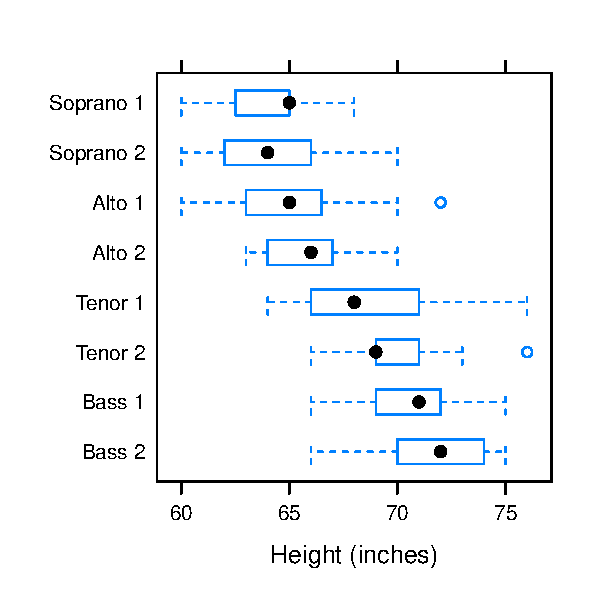
\includegraphics[width=\maxwidth]{figure/intro-pkg-1} 

}

\caption[Using the lattice package to create boxplots]{Using the lattice package to create boxplots}\label{fig:intro-pkg}
\end{figure}

\end{knitrout}


When you want to finish your session, just type \code{quit()}.

